%% bare_conf.tex
%% V1.3
%% 2007/01/11
%% by Michael Shell
%% See:
%% http://www.michaelshell.org/
%% for current contact information.
%%
%% This is a skeleton file demonstrating the use of IEEEtran.cls
%% (requires IEEEtran.cls version 1.7 or later) with an IEEE conference paper.
%%
%% Support sites:
%% http://www.michaelshell.org/tex/ieeetran/
%% http://www.ctan.org/tex-archive/macros/latex/contrib/IEEEtran/
%% and
%% http://www.ieee.org/

%%*************************************************************************
%% Legal Notice:
%% This code is offered as-is without any warranty either expressed or
%% implied; without even the implied warranty of MERCHANTABILITY or
%% FITNESS FOR A PARTICULAR PURPOSE! 
%% User assumes all risk.
%% In no event shall IEEE or any contributor to this code be liable for
%% any damages or losses, including, but not limited to, incidental,
%% consequential, or any other damages, resulting from the use or misuse
%% of any information contained here.
%%
%% All comments are the opinions of their respective authors and are not
%% necessarily endorsed by the IEEE.
%%
%% This work is distributed under the LaTeX Project Public License (LPPL)
%% ( http://www.latex-project.org/ ) version 1.3, and may be freely used,
%% distributed and modified. A copy of the LPPL, version 1.3, is included
%% in the base LaTeX documentation of all distributions of LaTeX released
%% 2003/12/01 or later.
%% Retain all contribution notices and credits.
%% ** Modified files should be clearly indicated as such, including  **
%% ** renaming them and changing author support contact information. **
%%
%% File list of work: IEEEtran.cls, IEEEtran_HOWTO.pdf, bare_adv.tex,
%%                    bare_conf.tex, bare_jrnl.tex, bare_jrnl_compsoc.tex
%%*************************************************************************

% *** Authors should verify (and, if needed, correct) their LaTeX system  ***
% *** with the testflow diagnostic prior to trusting their LaTeX platform ***
% *** with production work. IEEE's font choices can trigger bugs that do  ***
% *** not appear when using other class files.                            ***
% The testflow support page is at:
% http://www.michaelshell.org/tex/testflow/

\documentclass[sigplan,10pt]{acmart}

\usepackage[utf8]{inputenc}
\usepackage{listings}
\usepackage{todonotes}
\usepackage{comment}
\usepackage{url}
\usepackage{textcomp}
\usepackage{multirow}
\usepackage{booktabs}

\settopmatter{printfolios=true}

\graphicspath{{./data/img/}}

% Copyright
%\setcopyright{none}
%\setcopyright{acmcopyright}
%\setcopyright{acmlicensed}
\setcopyright{rightsretained}
%\setcopyright{usgov}
%\setcopyright{usgovmixed}
%\setcopyright{cagov}
%\setcopyright{cagovmixed}


% DOI
%\acmDOI{10.475/123_4}

% ISBN
%\acmISBN{123-4567-24-567/08/06}

%Conference
\acmConference[PLATEAU 2017]{8th Workshop on Evaluation and Usability of Programming Languages and Tools}{October 2017}{Vancouver, Canada}
\acmYear{2017}
\copyrightyear{2017}

%\acmPrice{15.00}

%\acmBadgeL[http://ctuning.org/ae/ppopp2016.html]{ae-logo}
%\acmBadgeR[http://ctuning.org/ae/ppopp2016.html]{ae-logo}



\begin{document}
%
% paper title
% can use linebreaks \\ within to get better formatting as desired
\title{OpenMP is Not as Easy as It Appears}

\begin{comment}
\author{
    \IEEEauthorblockN{Author 1\IEEEauthorrefmark{1}\IEEEauthorrefmark{2}, Author 2\IEEEauthorrefmark{2}, Author 3\IEEEauthorrefmark{2}, Author 4\IEEEauthorrefmark{2} and Author 5\IEEEauthorrefmark{2}}
    \IEEEauthorblockA{\IEEEauthorrefmark{1}Institution 1 Line 1\\
    Institution 1 Line 2\\
    Institution 1 Line 3\\
    author1@email}
    \IEEEauthorblockA{\IEEEauthorrefmark{2}Institution 2 Line 1\\
    Institution 2 Line 2\\
    Institution 2 Line 3\\
    Institution 2 Line 4\\
    \{author1, author2, author3, author4, author5\}@email}
}
\end{comment}

\author{
    \IEEEauthorblockN{Rogério Gonçalves\IEEEauthorrefmark{1}\IEEEauthorrefmark{2}, Marcos Amaris\IEEEauthorrefmark{2}, Thiago Okada\IEEEauthorrefmark{2}, Pedro Bruel\IEEEauthorrefmark{2} and Alfredo Goldman\IEEEauthorrefmark{2}}
    \IEEEauthorblockA{\IEEEauthorrefmark{1}Department of Computer Science -- DACOM\\
    Federal Technological University of Paraná -- UTFPR\\
    Campo Mourão/PR, Brazil\\
    rogerioag@utfpr.edu.br}
    \IEEEauthorblockA{\IEEEauthorrefmark{2}Software Systems Laboratory -- LSS\\
    Institute of Mathematics and Statistics -- IME\\
    University of São Paulo -- USP\\
    São Paulo/SP, Brazil\\
    \{rag, amaris, thiagoko, phrb, gold\}@ime.usp.br}
}


% conference papers do not typically use \thanks and this command
% is locked out in conference mode. If really needed, such as for
% the acknowledgment of grants, issue a \IEEEoverridecommandlockouts
% after \documentclass

% for over three affiliations, or if they all won't fit within the width
% of the page, use this alternative format:
% 
%\author{\IEEEauthorblockN{Michael Shell\IEEEauthorrefmark{1},
%Homer Simpson\IEEEauthorrefmark{2},
%James Kirk\IEEEauthorrefmark{3}, 
%Montgomery Scott\IEEEauthorrefmark{3} and
%Eldon Tyrell\IEEEauthorrefmark{4}}
%\IEEEauthorblockA{\IEEEauthorrefmark{1}School of Electrical and Computer Engineering\\
%Georgia Institute of Technology,
%Atlanta, Georgia 30332--0250\\ Email: see http://www.michaelshell.org/contact.html}
%\IEEEauthorblockA{\IEEEauthorrefmark{2}Twentieth Century Fox, Springfield, USA\\
%Email: homer@thesimpsons.com}
%\IEEEauthorblockA{\IEEEauthorrefmark{3}Starfleet Academy, San Francisco, California 96678-2391\\
%Telephone: (800) 555--1212, Fax: (888) 555--1212}
%\IEEEauthorblockA{\IEEEauthorrefmark{4}Tyrell Inc., 123 Replicant Street, Los Angeles, California 90210--4321}}

% use for special paper notices
%\IEEEspecialpapernotice{(Invited Paper)}

% make the title area
\maketitle

%\begin{abstract}
%\boldmath
%The abstract goes here.
%\end{abstract}
\begin{abstract}
%\boldmath
This paper aims to show that knowing the core concepts related to a given parallel architecture is necessary to write correct code, regardless of the parallel programming paradigm used.
Programmers unaware of architecture concepts, such as beginners and students, often write parallel code that is slower than their sequential versions. It is also easy to write code that produces incorrect answers under specific conditions, which are hard to detect and correct.\\
The increasing popularization of multi-core architectures motivates the implementation of parallel programming frameworks and tools, such as OpenMP, that aim to lower the difficulty of parallel programming. OpenMP uses compilation directives, or \textit{pragmas}, to reduce the number of lines that the programmer needs to write. However, the programmer still has to know when and how to use each of these directives. 
The documentation and available tutorials for OpenMP give the idea that using compilation directives for parallel programming is easy. In this paper we show that this is not always the case by analysing a set of corrections of OpenMP programs made by students of a graduate course in Parallel and Distributed Computing, at University of São Paulo.
Several incorrect examples of OpenMP \textit{pragmas} were found in tutorials and official documents available in the Internet. The idea that OpenMP is easy to use can lead to superficial efforts in teaching fundamental parallel programming concepts. This can in its turn lead to code that does not develop the full potential of OpenMP, and could also crash inexplicably due to very specific and hard-to-detect conditions. Our main contribution is showing how important it is to teach core architecture and parallel programming concepts properly, even when you have powerful tools such as OpenMP available.
% Institution 2 = University of São Paulo
\end{abstract}
% IEEEtran.cls defaults to using nonbold math in the Abstract.
% This preserves the distinction between vectors and scalars. However,
% if the conference you are submitting to favors bold math in the abstract,
% then you can use LaTeX's standard command \boldmath at the very start
% of the abstract to achieve this. Many IEEE journals/conferences frown on
% math in the abstract anyway.

% no keywords

% For peer review papers, you can put extra information on the cover
% page as needed:
% \ifCLASSOPTIONpeerreview
% \begin{center} \bfseries EDICS Category: 3-BBND \end{center}
% \fi
%
% For peerreview papers, this IEEEtran command inserts a page break and
% creates the second title. It will be ignored for other modes.
\IEEEpeerreviewmaketitle

%\section{Introduction}
% no \IEEEPARstart
%This demo file is intended to serve as a ``starter file''
%for IEEE conference papers produced under \LaTeX\ using
%IEEEtran.cls version 1.7 and later.
% You must have at least 2 lines in the paragraph with the drop letter
% (should never be an issue)
%I wish you the best of success.
%\hfill mds
%\hfill January 11, 2007
%\subsection{Subsection Heading Here}
%\subsubsection{Subsubsection Heading Here}
%Subsubsection text here.

\section{Introduction}
\label{sec:introduction}

There is an ongoing evolution of parallel processing platforms. The pursuit for high performance in general-purpose and scientific applications have turned to the exploration of the parallel processing capabilities provided by multi-core processors and arrangements of coprocessors like the Xeon Phi~\cite{xeonphiRuntime}. The machine currently at the top of the \textit{TOP500} list~\cite{dongarra1997top500} uses multi-core processors (12 cores) and Xeon Phi coprocessors~\cite{top500:site}.
Multi-core processors have become popular on personal computers and mobile devices. This popularization increases the need for specialized developers able to work in parallel applications and apply parallel computing models~\cite{Chen:2009:ChallengesMIC}~\cite{okur2012developers}.

Today there is a wide gap between legacy code applications that could benefit from parallel computing power and the new parallel computing platforms that could provide that power. However, legacy applications are generally sequential and therefore not easily scalable to multi-core architectures and parallel computing platforms. 

Asanovic \textit{et al.} \cite{Asanovic2009} describes this scenario, and defends the need for Structural and Computational Patterns in Parallel Computing. These patterns allow the portability of parallel programming solutions, while also allowing specialization of applications with the same behavior. In some situations it is not a matter of achieving the highest possible performance, but instead of making the application achieve acceptable performance, benefiting from a new parallel computing platform~\cite{Asanovic2009}. A similar approach is proposed by Pllana \textit{et al.} in a development environment that uses a combination of Model-Driven Development and Parallel Building Blocks \cite{Pllana:2009}. The approach consists in creating the model and then generating or transforming the code using \emph{model-to-source} tools.

In this context, the approach of using Compilation Directives to guide the compiler in the parallelization process has gained popularity. These directives are implemented using the compiler's pre-processing directives and are utilized as annotations that provide tips about the sequential code. Among the tools and extensions that use compilation directives are the \texttt{OpenMP} API \cite{Dagum1998a} \cite{Chapman:2007} used for writing programs for multi-core architectures, and the \texttt{OpenACC} programming standard~\cite{openacc:api}, used for writing programs for heterogeneous CPU/GPU architectures. The \texttt{OpenMP 4.0} specification supports offloading capabilities \cite{openmp:api:2013} such as \texttt{OpenACC} and \texttt{AMD HSA}~\cite{amd:hsa:site}. These tools aim to make easier the task of designing and implementing efficient and provably correct parallel algorithms. However, the abstraction layers built by the extensions also have the potential to conceal architectural details and to generate new parallel programming challenges.

When comparing \texttt{OpenMP} to other available tools for developing multi-threaded applications such as the \texttt{pthreads} interface, the API can be considered almost costless. However, when writing more complex applications this may not be true. The design and implementation of such complex applications require more knowledge about platforms and execution models than what can be shown by tutorials, that present high level and trivial examples. These tutorials try to convince the user that programming with directives is simple and easy to do, which is not always true. For instance, to achieve good performance in some cases it is necessary to describe many restrictions on annotations~\cite{OpenMPTasks2009}~\cite{mattson2003good}.

Krawezik and Cappello~\cite{CPE:CPE905} evidenced this difficulty by comparing MPI and three OpenMP versions of benchmarks. The most popular use of \texttt{OpenMP} directives is at the loop level. The programmer discovers potentially parallel loops and annotates the code with directives starting and closing parallel regions. Good results were obtained only when SPMD was implemented on OpenMP, and achieving good performance required a significant programming effort~\cite{CPE:CPE905}.

In this work we have gathered data from assignments made by graduate students for the \emph{Introduction to Parallel and Distributed Computing} course. Among other exercises, the students were asked to find examples of \texttt{OpenMP} code in tutorials and official manuals that failed under special conditions. These conditions could be created by, for example, placing barriers or forcing racing conditions by exposing inaccurate thread management.

We argue that it is necessary to consider fundamental concepts of architectures and parallel programming techniques when teaching students new to the subject, so that they can learn when and how to apply the programming models~\cite{ben1999thinking}. The abstractions provided by parallel programming tools over concepts such as threads, barriers and loop parallelization should be carefully studied, analysed and conceptually built in the classroom before they are used by the students in their assignments.

We found eight tutorials with different kinds of \texttt{OpenMP} errors in the experiment with the students' assignments. Many of these errors where similar to the most common \texttt{OpenMP} mistakes~\cite{SuB:2005:CMO:1892830.1892863}. The most common type of error identified in our experiment was the management of shared or private variables. This problem is common across multiple programming paradigms.

The \textbf{main contribution of this work} is to show the importance of teaching core architecture and parallel programming concepts thoroughly, despite the availability of powerful tools such as \texttt{OpenMP}. We also aim to show that the \texttt{OpenMP} API is not as easy to use as it might seem.

The rest of the paper is organized as follows. The following section discusses related work. Section~\ref{sec:concurrency} discusses concurrency and other concepts in parallel computing. Section~\ref{sec:directives} presents the idea of compilation directives. Section~\ref{sec:methodology} discusses the methodology applied in the experiments, and Section~\ref{sec:results} presents our results. Section~\ref{sec:students:perception} presents the perceptions of the graduate students regarding the exercise and learning \texttt{OpenMP}. Finally, Section~\ref{sec:conclusions} presents the conclusions and next steps.

% Institution 2 = University of São Paulo

\section{Related Work}
\label{sec:relatedwork}

There has been a large body of works that have presented results of studies and experiments in teaching parallel computing courses. S\"{u}\ss~and Leopold~\cite{SuB:2005:CMO:1892830.1892863} discuss the teaching of parallel computing, in particular the use of \texttt{OpenMP}. The authors present the most common errors identified in assignments given in parallel computing classes. The errors were classified in two categories: \emph{correctness mistakes} and \emph{performance mistakes}. Errors that impact the correctness of a program are errors of the first category. Errors which make programs perform slower are classified in the second category. The work also provides a checklist containing tips to avoid the most common mistakes.

Falcao~\cite{6565518} defends that teaching a parallel programming model or interface such as \texttt{OpenMP} in the beginning of undergraduate courses is not much harder than teaching a language like C or C++. The benefits of teaching these skills early on in the course would be interesting, considering that the majority of computer architectures are now are multi-core. Parallel computing should be taught with the use of higher level tools. One of the approaches proposed by Ferner \textit{et al.}~\cite{6651019} is to use compiler directives to describe how a program should be parallelized.

The need for Structural and Computational Patterns to Parallel Computing is defended by Asanovic \textit{et al.}~\cite{Asanovic2009} as the way to allow portability of solutions and the specialization of applications with the same behavior. Using patterns to design applications make it easy to change the target platform. The applications will be bound to platforms in low levels of architecture and probably inside a specialized function which can be easily changed. 

A similar approach is proposed by Pllana \textit{et al.}~\cite{Pllana:2009} in a programming environment that uses a combination of Model-Driven Development and Parallel Building Blocks. The idea is to create the model and then generate or transform the code using model-to-source tools. The proposed environment uses intelligent agents to assist the programmer, this is done during the high level program composition and when the programmer loads a BLAS function for some dense linear algebra operation, the tool suggests the use of the appropriate parallel basic block. The parallelism is inside the parallel building blocks and the programmer is not exposed directly to the complexity of parallel programming problems.

Speyer \textit{et al.}~\cite{4755913} defend that implementing applications with high performance is harder than ever, specially due to the emergence of multi-core architectures. This leads to the development of hybrid applications that use both the \texttt{OpenMP} and \texttt{MPI} (\emph{Message Passing Interface}) APIs. This presents even greater challenges to the programmers, since they now need to know how to use both code annotations and message passing abstractions to achieve high performance. The paper then compares different parallel programming tools with regard to their ease of use. There is a substantial effort to start writing parallel and high performance code even with these tools.

Some problems can be solved using different directive combinations, and the chosen combination influences the code that is generated. The \texttt{Parallware}~\cite{Parallware:2014} source-to-source compiler showed how different strategies and uses of directive combinations can lead to different performance results. The use of the wrong \texttt{OpenMP} directives and strategies can significantly reduce the performance over a sequential version.

The \texttt{OmpVerify}~\cite{Basupalli:2011} system implements a static analysis tool based on the polyhedral model to extract the parallel portions of a program automatically and to detect important classes of common data-race errors in \texttt{OpenMP} \texttt{parallel for} directives. Saillard \textit{et al.}~\cite{Saillard:2014} statically validates barriers and work sharing constructs to avoid the improper use of directives that could cause deadlocks. S\"{u}\ss~and Leopold~\cite{Leopold:userOpenMP}, present an user's experience with parallel sorting and OpenMP. They have used several versions of a simple parallel sorting algorithm to show some weaknesses of OpenMP.

Substantial efforts have been made to achieve the simplest possible way to parallelize code, and the task is not easy. In this paper we present an exploratory analysis of common \texttt{OpenMP} errors, confirming that programming with high-level APIs and abstractions can still be difficult.

\section{Concurrency and Multithreading Programming}
\label{sec:concurrency}

A program is composed of data declarations, assignments and control flow, following the syntax and abstractions of a programming language. A concurrent program is a set of sequential programs that can be executed in parallel~\cite{Ben-Ari:1990}.

In 2004, the first multi-core processor was launched~\cite{Sutter:2005} into the mainstream market. The increasing number of cores of current parallel machines has motivated concurrent execution of tasks in all scientific and commercial domains, although this paradigm may still face some resistance~\cite{FreeLunchIsOver} \cite{threadsProblem:2006} \cite{KISS:2004:article}. Two important concepts are \emph{concurrency} and \emph{parallelism}. Concurrency occurs when multiple tasks are logically active at the same time and parallelism occurs when multiple tasks are actually active at the same time. In this case parallelism is related to physically performing tasks in parallel. In a computer with a multi-core processor we can have physical parallelism.

In practically every language that supports multi-threading, the implementation of this concept follows the idea of having a function with the code to be executed by the thread when it is created. Programming multi-threaded applications is a complex task, independently of the language used. The non determinism that is introduced by the use of threads can be controlled using synchronization mechanisms such as locks \cite{threadsProblem:2006}, semaphores and barriers, but these mechanisms increase the complexity of the program even more. 

In C/C++ languages the \texttt{pthreads} library can be used to control thread execution on GNU/Linux. This library implements the standard POSIX API (IEEE 1003.1c) and provides mechanisms to create and synchronize threads. The choice to use the \texttt{pthreads} library, and not \texttt{OpenMP}, can be motivated by the fact that \texttt{pthreads} is a common library, available on platforms with GNU/Linux, and operates in a lower level of abstraction in comparison with \texttt{OpenMP} threads. The Code~\ref{cod:sample:pthreads} presents a sample of code that uses the \texttt{pthreads} library.

\begin{lstlisting}[style=C, label=cod:sample:pthreads,caption=The Sample of pthreads code.]
int main(){
  pthread_t thread1;
  DATA_TYPE *params = 10;
  int iret1;

  iret1 = pthread_create( &thread1, NULL, task_function, (void*) params);
  printf("Thread 1 return: %d\n", iret1);
  pthread_join(thread1, NULL);
  
  return 0;
}

void *task_function(void *ptr) {
  DATA_TYPE *value;
  value = (DATA_TYPE *) ptr;
  /* Computing */
}
\end{lstlisting}

This sample code shows some important concepts. Until \texttt{line 6} only one thread is executing the main flow of instructions. When the \texttt{pthread\_create()} function is called, a new thread is created and then the application have two threads executing in parallel. For synchronization between threads barriers are necessary. The library implements barriers and they can be used in the code by calling \texttt{pthread\_join()}. In \texttt{line 8} we can see an example of this, where the thread that reaches that point will wait for the completion of other threads to continue the execution of the main flow.

To explain the use of \texttt{pthreads} we use the sample code in Code~\ref{cod:basic} to create a parallel version. The code have a reduction operation, in the multiplication of elements of $A$ and $B$ to the $dot$ variable. In this case, we want to parallelize the loop instances by dividing the amount of instances among a number of threads.

\begin{lstlisting}[style=C, label=cod:basic,caption=Sample of Basic Code.]
 for(i = 0; i < N; i++){
   dot += A[i] * B[i];
 }
\end{lstlisting}

The Code~\ref{cod:sample:vetdot:pthreads} shows a vector product operation that was implemented using \texttt{pthreads}. This example shows that we need to write several lines of code to perform a simple operation like sharing work between threads.

% float=ht 
\begin{lstlisting}[style=C, label=cod:sample:vetdot:pthreads,caption=The vetdot sample using pthreads.]
int A[SIZE], B[SIZE];
int dot = 0;

pthread_mutex_t lock;

int main( int argc, char *argv[] ){
  int num_threads, i, part_size;
  
  pthread_t tid[MAX_THREADS];
	
  pthread_attr_t attr;
  pthread_attr_init(&attr);
	
  /* Initialization vectors was supressed. */
	
  part_size = (SIZE + num_threads - 1) / num_threads;
	
  for (i=0; i < num_threads; i++) {
  	struct arg_struct *args = malloc(sizeof(struct arg_struct));
		
  	args->id = i;
  	args->i_part = (i * part_size);
  	args->e_part = MIN(((i + 1)* (part_size)), SIZE);
  	
  	pthread_create(&(tid[i]), &attr, vecDot, (void *) args);
  }
	
  for (i=0; i<num_threads; i++) {
  	pthread_join(tid[i], NULL);
  }
	
  printf("Final result: %d.\n", dot);
	
  return 0;
}

void *vecDot(void *arguments){
  struct arg_struct *args = arguments;
  int i, partial_dot = 0;	
	
  for(i = args->i_part; i < args->e_part; i++){ 
  	partial_dot += A[i] * B[i]; 
  }
	
  /* Critical region. */
  pthread_mutex_lock(&lock);
  dot += partial_dot;
  pthread_mutex_unlock(&lock);
	
  pthread_exit(0);
}
\end{lstlisting}

In the main function, the arrays are initialized and divided among the number of created threads. Each thread executes the \texttt{vetDot} function, saving the calculated $partial\_dot$ value in the global $dot$ variable. This is done inside a delimited critical region, defined by the use of using \textit{pthread} \textit{mutexes}.

\section{Compilation Directives}
\label{sec:directives}

Since the introduction of heterogeneous parallel computing platforms tools have been developed to provide interfaces between compilers, runtimes and execution environments. The compilation directives is one of the approaches that has excelled in the context of parallel computing, because annotating code is usually easier than rewriting it. These directives are commonly implemented using the pre-processing directives \texttt{\#pragma}, in \texttt{C/C++}, and sentinels \texttt{!\$}, in the Fortran language.

Directives are used as annotations that provide tips about the original code and guide the compiler in the parallelization process of candidate regions. During the pre-processing, the \textit{tokens} that compose the directive can be replaced using macros, for example. The parallel version of the code will use features provided by the \texttt{OpenMP} runtime.

%\url{http://www.google.com/trends/explore#cat=0-5&q=openmp%2C%20hpf&cmpt=q&tz=Etc%2FGMT%2B3}
The use of directives was not introduced by \texttt{OpenMP}. Directives have been used as a macro specification language used in the pre-processing of languages such as C/C++ and Fortran. The macros transform the source code before the compilation. Languages such as \texttt{HPF} \cite{Richardson96highperformance} \cite{hpf:1997} had compiler directives for parallelism before the rise of \texttt{OpenMP}. However, with the popularity of multi-core processors and \texttt{OpenMP} supporting C/C++ and Fortran applications, \texttt{OpenMP} has become a robust runtime for multi-core processors and an interesting application of compilation directives. Figure~\ref{fig:google:trends:openmp} presents a comparison between the search results for the terms \lq\lq\texttt{OpenMP}\rq\rq{}, \lq\lq\texttt{HPF}\rq\rq{} (High Performance Fortran) and \lq\lq\texttt{Cilk}\rq\rq. The constantly higher number of searches for \lq\lq\texttt{OpenMP}\rq\rq{} can be taken as confirmation of its popularity.

\begin{figure}[htpb]
\centering
\includegraphics[width=1\columnwidth,height=0.35\columnwidth]{figures/google-trends-openmp.pdf}
\caption{Comparison of the Google Trends results for \lq\lq\texttt{OpenMP}\rq\rq, \lq\lq\texttt{HPF}\rq\rq{} and \lq\lq\texttt{Cilk}\rq\rq.}
\label{fig:google:trends:openmp}
\end{figure}

Using compilation directives is interesting because legacy code applications can be annotated and then parallelized by the runtime, to achieve performance improvements on multi-core processors. If the annotated code is analyzed by a compiler that supports \texttt{OpenMP} \cite{Dagum1998a} \cite{openmp:api:2011} \cite{openmp:api:2013} \cite{Chapman:2007} \cite{openmp:site}, a parallel version will be generated. Otherwise, the directives will be ignored and the code will remain sequential. Using the \texttt{OpenMP} runtime, parallel C/C++ or Fortran programming requires only the learning the directives' usage.

\texttt{OpenMP} is a set of compilation directives, functions libraries and environment variables that are based on the C/C++ and Fortran languages. The high level directives are able to expose the low level parallelism resources available on native implementations like the \texttt{pthreads} interface on GNU/Linux. Using the \texttt{OpenMP} directives much of the work is done automatically and implicitly, parallel regions have implicit barriers and the declaration of shared or private variables is simple.

\texttt{OpenMP} implements the \texttt{fork-join} model, in which multiple threads of execution perform tasks defined implicitly or explicitly by \texttt{OpenMP} directives~\cite{openmp:api:2011}~\cite{openmp:api:2013}. Threads are created from annotated code blocks. The \textit{master thread} executes sequentially until it finds the first parallel region. The similar \texttt{fork} operation creates a team of threads to execute a parallel region, the \textit{master thread} is part of the team. Nested parallel regions are allowed. When all threads in a team reach the barrier that marks the end of the parallel region, the master thread continues until it finds a new parallel region. From the annotated blocks, the runtime can generate implicit threads to execute the parallel regions or assign to some other thread the execution of explicit tasks defined by the programmer using the \texttt{task} directive.

Multiple compilers implement \texttt{OpenMP}, such as \texttt{GCC} \cite{libgomp:2015} and LLVM \texttt{clang} \cite{LLVM:CGO04} \cite{clang:site} \cite{openmp:llvm:site}, for example. \texttt{OpenMP} is certainly easier to use than \texttt{pthreads}~\cite{CPE:CPE529}. The directives allow a first contact with parallel programming that uses basic examples, letting the programmer experience an effortless application of parallel computing. However, complex parallel programming require more than simple \texttt{OpenMP} directives. Code~\ref{cod:sample:openmp} presents an example of the \texttt{OpenMP} compilation directives used to compute the dot product, which can be compared to a \texttt{pthreads} version presented in Code~\ref{cod:sample:vetdot:pthreads}.

\begin{lstlisting}[style=C, label=cod:sample:openmp,caption=Sample of OpenMP code.]
#pragma omp parallel firstprivate(aux_dot)
{
  #pragma omp single
  printf("Begin of the parallel region, number of threads: %d\n", omp_get_num_threads());
    
  #pragma omp for schedule(runtime)
  for(i = 0; i < SIZE; i++){ 
    aux_dot += A[i] * B[i];
  }
    
  #pragma omp critical
  dot += aux_dot;
    
  #pragma omp master
  printf("Final result: %d.\n", dot);
}
\end{lstlisting}

Expanding the code with directives allows to see how \texttt{OpenMP} reduces the amount of code that the programmer needs to write. The code with the expansions is shown in Code~\ref{cod:expanded:openmp}.

\begin{lstlisting}[style=C, label=cod:expanded:openmp,caption=OpenMP expanded code]
long long A[SIZE], B[SIZE], dot = 0;

void subfunction0 (void *data) {
  long long aux_dot = 0;
  
  if (GOMP_single_start ())
    printf("Begin of the parallel region, number of threads: %d\n", omp_get_num_threads());
  GOMP_barrier ();
  
  {
    long i, _s0, _e0;
    if (GOMP_loop_runtime_start (0, SIZE, 1, &_s0, &_e0))
      do {
        long _e1 = _e0;
        for (i = _s0; i < _e0; i++){
          aux_dot += A[i] * B[i];
        }
      } while (GOMP_loop_runtime_next (&_s0, &_e0));
    GOMP_loop_end ();
  }
  
  GOMP_critical_start();
  dot += aux_dot;
  GOMP_critical_end();
    
  if (omp_get_thread_num () == 0)
    printf("Final result: %d.\n", dot);
}

int main() {
  /* Initializations were supressed. */

  GOMP_parallel_start (subfunction0, NULL, 2);
  subfunction0 (NULL);
  GOMP_parallel_end ();

  return 0;
}
\end{lstlisting}

The Code~\ref{cod:expanded:openmp} shows calls to \texttt{GOMP\_parallel\_start()} \texttt{(line 33)} and \texttt{GOMP\_parallel\_end()} \texttt{(line 35)}. These functions are responsible to start and finish the team of threads that run \texttt{subfunction0(...)}. In the code it is also possible to see the functions that are mapped to barriers and synchronization. The calls to \texttt{GOMP\_barrier()} in \texttt{line 8}, \texttt{GOMP\_critical\_start()} and \texttt{GOMP\_critical\_end()} in \texttt{lines 22} and \texttt{24}, are mapped to semaphore and barrier primitives that are implemented in specific \texttt{OpenMP} libraries. 

The \texttt{OpenMP} runtime uses the standard thread library of the system, in this case, \texttt{pthreads}. The library is used together with other native system resources to control scheduling and synchronization. This shows that \texttt{OpenMP} is simpler comparing to code using \texttt{pthreads}, but the programmer still needs to master fundamental concepts about parallelism.

Tutorials present content in a structured way, showing the syntax of directives and exemplifying the use of annotations. The examples are simple in most cases, as can be seen in Code~\ref{cod:sample:openmp}. This kind of example brings to student the idea that \texttt{OpenMP} is always very simple. They simply annotate the code and make the program parallel.
In simple applications, we write one or two annotations in the code and generate a parallel version without difficulty. However, when we have more complex applications, it is necessary to know more concepts of parallel computing to apply the correct modifications in the source code. 

Another common situation when using compilation directives is obtaining a better performance for a parallel version of the code. It is necessary to perform large efforts to include the annotations and their proper restrictions. That turns the process into something like \lq\lq{}annotation or directive oriented programming\rq\rq. The time gained by not rewriting the application code is spent declaring directives and their restrictions.

Krawezik and Cappello~\cite{CPE:CPE905} evidenced this difficulty by comparing MPI and three OpenMP versions of benchmarks. The most popular use of \texttt{OpenMP} directives is at the loop level. In this approach the programmer discovers potentially parallel loops by profiling and checking the dependencies. The programmer then annotates the code with directives starting and closing parallel regions at each discovered parallelizable loop. However, good results were obtained only when SPMD was implemented on \texttt{OpenMP}, and achieving good performance required a significant programming effort~\cite{CPE:CPE905}.


\section{Methodology}
\label{sec:methodology}

% Institution 2 = University of São Paulo

The motivation to write this paper comes from experiences on teaching. During the classes of Distributed Systems and Parallel Programming, a graduate course at University of São Paulo, a problem was detected in an \texttt{OpenMP} code sample.

To explain the idea we use as a basis the code sample showed in Code~\ref{cod:basic} of section \ref{sec:concurrency}. If we need to parallelize the loop instances, we can use the \texttt{OpenMP} \emph{reduction} clause because the code has a \emph{reduction} operation, but the idea of the tutorial was to show the use of the \emph{critical} clause.

The code written on the tutorial sample to solve using \emph{critical} clause is shown in Code~\ref{cod:tutorial:sample:with:problem}. However, this code has a problem. 
 
\begin{lstlisting}[style=C, label=cod:tutorial:sample:with:problem,caption=Code of original OpenMP tutorial with problem.]
#pragma omp parallel
{
  #pragma omp for
  for(i = 0; i < N; i++){
   aux_dot += A[i] * B[i];
  }
  #pragma omp critical
  dot += aux_dot;
}
\end{lstlisting}

The idea that was used to parallelize the computing on \texttt{line 5} was to put the for loop inside a parallel region and parallelize the instances of the loop using the directive \texttt{\#pragma omp for}. An auxiliary variable $aux\_dot$ was used to keep the partial results in each thread, but $aux\_dot$ was not declared as private to each thread. This generated a race condition, in which threads can read the same value and can be interrupted before storing the updated value.

This situation was identified as a possible problem. In the second tutorial the authors thought the problem was in the initialization of the variable $dot$. The code was \lq\lq{}fixed\rq\rq{} using the \texttt{firstprivate(dot)} clause. The semantic of this clause is: \lq\lq{}all variables in the list are initialized with the original value before entering the parallel region\rq\rq{}. Code~\ref{cod:tutorial:sample:proposed:correction:1} presents the first attempt to fix the code in the class.
 
\begin{lstlisting}[style=C, float=htpb, label=cod:tutorial:sample:proposed:correction:1,caption=The first version of "fixed" code.]
#pragma omp parallel firstprivate(dot)
{
  #pragma omp single
  printf("Begin of the parallel region, number of threads: %d\n", omp_get_num_threads());
  #pragma omp for
  for(i = 0; i < SIZE; i++){
    aux_dot += A[i] * B[i];
    printf("Thread %d executes the loop iteration %02d: %lld * %lld = %lld -> %lld \n", omp_get_thread_num(), i, A[i], B[i], (A[i] * B[i]), aux_dot);
  }
  #pragma omp critical
  dot += aux_dot;
  
  #pragma omp master
  printf("Final result: %lld.\n", dot);
}
\end{lstlisting}

% Critical sections don't have barriers, neither at their beginnings nor at their ends. A critical section is a synchornisation construct on its own that prevents multiple threads from accessing the same data concurrently. You need an additional barrier after the critical section if you'd like to have the correct global minimum before you exit the parallel region. As was already said the parallel region has an implicit barrier at the end.

The author added lines on the code to show the final result, but with these modifications a new error was inserted. Only by the master thread prints the final result message, and this can occur before the completion of other threads, because the \emph{critical} clause does not have barriers, it only prevents concurrent accesses. The corrected code still had problems. One team of students found another problem in the \lq\lq{}fixed\rq\rq{} version of sample code. Code~\ref{cod:tutorial:sample:proposed:correction:2} presents the fixed and final code version.
 
\begin{lstlisting}[style=C, float=htpb, label=cod:tutorial:sample:proposed:correction:2,caption=The final version of code sample.]
#pragma omp parallel firstprivate(aux_dot)
{
  #pragma omp single
  printf("Begin of the parallel region, number of threads: %d\n", omp_get_num_threads());
  #pragma omp for
  for(i = 0; i < SIZE; i++){
    aux_dot += A[i] * B[i];
    printf("Thread %d executes the loop iteration %02d: %lld * %lld = %lld -> %lld \n", omp_get_thread_num(), i, A[i], B[i], (A[i] * B[i]), aux_dot);
  }
  #pragma omp critical
  dot += aux_dot;
}
printf("Final result: %lld.\n", dot);
\end{lstlisting}
 
The last correction puts the final message out of the parallel region to avoid printing incomplete results. This occurs because at the end of all parallel regions in OpenMP there is one implicit barrier that joins the work flow and only the \texttt{master thread} continues the execution in this case.

% Para nossa surpresa, não apenas um dos nossos exemplos em sala estava com problemas, mas erros foram encontrados em diversos tutoriais disponíveis na internet.

This simple example illustrates how mistakes can be made. The example motivated the proposition of an exercise for the students. It also reinforced the importance of fundamental parallelism concepts even in simpler approaches. A challenge was then proposed for the students, as one of the activities of the course. 
After the introductory lecture on \texttt{OpenMP}, the groups should search available \texttt{OpenMP} tutorials on the Internet for errors, and fix them. This exercise had $27$ participants, the group of students was divided in $6$ teams of two students and other students preferred to work alone. Most students used the \texttt{GCC} compiler and the \texttt{GNU libgomp} library in their assignments.

We applied a questionnaire to obtain more information about the students. Most students already knew threads, but few students had experience with \texttt{OpenMP}. Figure~\ref{fig:students:experience} presents how many students had contact with each parallel programming paradigms before the course. Since this is a graduate level course, we had students of various ages. This is reflected by the large differences in experience time between students, showed in Figure~\ref{fig:DifOpenMP}.

\begin{figure}[htpb]
\centering
% \includegraphics[width=0.95\columnwidth,height=0.65\columnwidth]{figures/experiencePP.eps}
\includegraphics[width=1.0\columnwidth,height=0.70\columnwidth, trim={0 1.0cm 0 1.5cm},clip]{figures/experiencePP.pdf}
\caption{APIs for Parallel Programming previously used by the students}
\label{fig:students:experience}
\end{figure}

The other question was about the programming languages known by the students. The objective of this information was to measure how easy it is to learn \texttt{OpenMP} when you know the basic concepts and what is the influence that the knowledge of other languages can have on the process. Figure~\ref{fig:LangMoreUsed} presents the distribution of programming languages known for the students involved in the experiment.

\begin{figure}[htpb]
\centering
% \includegraphics[width=0.95\columnwidth,height=0.65\columnwidth]{figures/experienceLP.eps}
\includegraphics[width=1.0\columnwidth,height=0.70\columnwidth, trim={0 1.0cm 0 1.5cm},clip]{figures/experienceLP.pdf}
\caption{Programming Languages more used by the students}
\label{fig:LangMoreUsed}
\end{figure}

\section{Results}
\label{sec:results}

After the students submitted the assignment for evaluation, we analyzed the reports and tutorials where errors were found. One of the examples shown in class presented an error, and multiple errors were found in several tutorials available on the Internet. Table~\ref{table:tutorials:with:problems} summarizes the errors found in tutorials from the Internet and their corrections by the students.
\begin{table}[ht]
\renewcommand{\arraystretch}{1.3}
\caption{Tutorials that presented some problem}
\label{table:tutorials:with:problems}
\centering
\begin{tabular}{|>{\centering\arraybackslash} m{.2cm}|>{\centering\arraybackslash} m{1.7cm}|  >{\centering\arraybackslash} m{2.75cm}|>{\centering\arraybackslash} m{2.75cm} |}
\hline
\textbf{Id}&\textbf{Tutorial} & \textbf{Identified Problem} & \textbf{Correction}\\
\hline

\begin{minipage}[m]{0.02\columnwidth}%
\centering
1
\end{minipage}&
\begin{minipage}[t]{0.22\columnwidth}%
\texttt{Tutorial de OpenMP C/C++~\cite{LCCV:UFAL:Tutorial}}
\end{minipage}&
\begin{minipage}[t]{0.33\columnwidth}%
Incorrect result. Race condition in results variables was detected.
\end{minipage}& 
\begin{minipage}[t]{0.33\columnwidth}%
The clause firstprivate was used to transform $aux\_dot$ in private variable in threads. \tiny{\texttt{\#pragma omp parallel firstprivate(aux\_dot)}}
\end{minipage}
\tabularnewline
\hline

\begin{minipage}[m]{0.02\columnwidth}%
\centering
2
\end{minipage}&
\begin{minipage}[t]{0.22\columnwidth}%
\texttt{Guide into OpenMP~\cite{OpenmpAndFork}}
\end{minipage}&
\begin{minipage}[t]{0.33\columnwidth}%
\texttt{OpenMP} interaction with Linux fork implementation using the GCC. The created thread pool are passed to child processes, but the fork() do not duplicate the threads causing deadlock in the child processes.
\end{minipage}&
\begin{minipage}[t]{0.33\columnwidth}%
Make fork() before application of pragmas in the parent process. Organize the code for child processes create their own thread pool.
\end{minipage}
\tabularnewline
\hline

\begin{minipage}[m]{0.02\columnwidth}%
\centering
3
\end{minipage}&
\begin{minipage}[t]{0.22\columnwidth}%
\texttt{Code Project~\cite{CodeProject}}
\end{minipage}&
\begin{minipage}[t]{0.33\columnwidth}%
Sintax error. Missing the~\lq\lq\{\rq\rq~after directive for.
\end{minipage}&
\begin{minipage}[t]{0.33\columnwidth}%
The students tested take off~\lq\lq\}\rq\rq~at the final causing segmentation fault error.
So they put the~\lq\lq\{\rq\rq~after the directive for.
\end{minipage}
\tabularnewline
\hline

\begin{minipage}[m]{0.02\columnwidth}%
\centering
4
\end{minipage}&
\begin{minipage}[t]{0.22\columnwidth}%
\texttt{Parallel Processing with OpenMP~\cite{BostonUniversity}}
\end{minipage}&
\begin{minipage}[t]{0.33\columnwidth}%
Error on use of ordered clause. It is necessary to indicate that the ordered clause will be used inside of loop.
\end{minipage}& 
\begin{minipage}[t]{0.33\columnwidth}%
The ordered clause was put.
\end{minipage}
\tabularnewline
\hline
\begin{minipage}[m]{0.02\columnwidth}%
\centering
5
\end{minipage}&
\begin{minipage}[t]{0.22\columnwidth}%
\texttt{Task Parallelism in OpenMP~\cite{UniversityUtah}}
\end{minipage}&
\begin{minipage}[t]{0.33\columnwidth}%
The $tid$ is not defined as private. It is shared by all threads the vector $A$ values are not calculated.
\end{minipage}&
\begin{minipage}[t]{0.33\columnwidth}%
Declare $tid$ as private using the \texttt{private(tid)} clause.
\end{minipage}
\tabularnewline
\hline
\begin{minipage}[m]{0.02\columnwidth}%
\centering
6
\end{minipage}&
\begin{minipage}[t]{0.22\columnwidth}%
\texttt{Introduction to Parallel Processing. OpenMP~\cite{UniversityEmory}}
\end{minipage}&
\begin{minipage}[t]{0.33\columnwidth}%
Use of \texttt{cout} function inside parallel region without critical clause. The threads are interrupted during the printing, messages are concatenated.
\end{minipage}&
\begin{minipage}[t]{0.33\columnwidth}%
The code was modified using the critical clause.
\end{minipage}
\tabularnewline
\hline
\begin{minipage}[m]{0.02\columnwidth}%
\centering
7
\end{minipage}&
\begin{minipage}[t]{0.22\columnwidth}%
\texttt{Introduction to Parallel and Distribution Systems. OpenMP Overview~\cite{UniversityWayne}}
\end{minipage}&
\begin{minipage}[t]{0.33\columnwidth}%
In the matrix multiplication code the variables $j$ and $k$ are shared by all threads generating wrong result.
\end{minipage}&
\begin{minipage}[t]{0.33\columnwidth}%
Addition of private clause on \tiny{\texttt{\#pragma omp parallel for private(j, k)}}
\end{minipage}
\tabularnewline
\hline
\begin{minipage}[m]{0.02\columnwidth}%
\centering
8
\end{minipage} &
\begin{minipage}[t]{0.22\columnwidth}%
\texttt{Introduction to OpenMP. Dijkstra sample~\cite{UniversityCalifornia}}
\end{minipage} & 
\begin{minipage}[t]{0.33\columnwidth}%
When the code is executed with more of 3 threads produces wrong results. There is an error in assigning values for $startv$ and $endv$ variables that keep the start and end positions of the shortest path. With this problem the algorithm does not reach all graph vertices. On line 88 a critical section is created for updating the minimum value and the vertex ($md$ and $mv$) but the code is not avoiding that updates occurs before another thread update the global vector, it is printing the values set in the initialization vector.
\end{minipage}&
\begin{minipage}[t]{0.33\columnwidth}%
The definition of variables $startv$ and $endv$ was modified using the original idea of algorithm. The \texttt{\#pragma omp barrier} directive was added after the \texttt{\#pragma omp critical}.
\end{minipage}
\tabularnewline
\hline

\end{tabular}
\end{table}

% Esses sites são os seguintes:
% http://bisqwit.iki.fi/story/howto/openmp/#OpenmpAndFork, 
% http://www.codeproject.com/Articles/60176/A-Beginner-s-Primer-to-OpenMP
% Universidade de Boston - www.bu.edu/tech/files/2011/09/openmp.ppt
% Tutorial disponiblizado pela Universidade de Utah, dado pelo seguinte link: http://www.cs.utah.edu/~mhall/cs4961f11/CS4961-L9.pdf.
% Tutorial da universidade de Emory (USA) OpenMP  http://www.mathcs.emory.edu/~cheung/Courses/355/Syllabus/91-pthreads/openMP.html
% Universidade do Estado de Wayne (USA) Apresentação de Cheng-Zhong Xu. site: http://www.ece.eng.wayne.edu/ czxu/ece561/lnotes/OpenMP.pdf
% Site de Question, Answer. http://askubuntu.com/questions/590755/openmp­unable­to­use­multiple­threads­no­error­a ssociated­with­compilation. Já tinha sido corregido.
% Universidade de California, Davis. Introduction to OpenMP.  http://heather.cs.ucdavis.edu/~matloff/openmp.html#tutorials. http://heather.cs.ucdavis.edu/~matloff/OpenMP/Examples/NM/Dijkstra.c

The \emph{first tutorial} in Table~\ref{table:tutorials:with:problems} has a problem caused by a confusion about which variables are shared and which should be private. This problem is similar to the ones identified by S\"{u}\ss~and Leopold~\cite{SuB:2005:CMO:1892830.1892863} as common correctness mistakes (\lq\lq{}Forgetting to mark private variables as such\rq\rq{}). It was the fourth most frequent mistake in that study.

\emph{Tutorial 2} presents a problem with the interaction between \texttt{OpenMP} and the system's OS and compiler. Specifically, the \texttt{GCC} \texttt{fork()} implementation. When we use the fork primitive, the Operating System creates other processes (child processes) duplicating all resources used by processes that execute the \texttt{fork()} call. Using \texttt{OpenMP} and creating child processes makes the thread pool created by \texttt{OpenMP} to be passed to child processes, but \texttt{fork()} does not duplicate the threads, which causes deadlock in the child processes.

The problem presented in \emph{tutorial 3} was a syntax error, there was a missing ~\lq\lq\{\rq\rq{} after the directive.

\emph{Tutorial 4}, presented in Table~\ref{table:tutorials:with:problems}, was found by students because of an error using the \texttt{ordered} clause. When using this clause it is necessary to indicate that it will be used inside a loop. A similar mistake involving the clause was identified as common by S\"{u}\ss~and Leopold~\cite{SuB:2005:CMO:1892830.1892863}. The opposite situation happened when an \texttt{ordered} clause was put into a \texttt{for} construct without being specified by a separate \texttt{ordered} clause inside the loop. This is a restriction on the nesting of regions, an \texttt{ordered} region must be closely nested inside a loop or parallel loop region with an \texttt{ordered} clause~\cite{openmp:api:2011}.

Other problems in private variable definition were found in \emph{tutorials 5} and \emph{7}. In \emph{tutorial 5} the \texttt{tid} variable is not defined as private, causing some values in the array not being calculated. In \emph{tutorial 7} the variables \texttt{j} and \texttt{k} in the matrix multiplication are shared by all threads, generating wrong results.

In \emph{tutorial 6} the \texttt{cout} function is called inside a parallel region without a protecting \texttt{critical} clause. The call becomes a critical section, because the threads are interrupted during the printing and messages are concatenated generating incorrect results. The code was modified by students using the \texttt{critical} clause to ensure that the call is executed by one thread at a time.

\emph{Tutorial 8} presents a synchronization problem that causes an error in the assignment of values for the \texttt{startv} and \texttt{endv} variables that keep the start and end positions of the shortest path. Because of this problem the algorithm does not reach all graph vertices. The critical section is created to update the minimum value and the vertex (\texttt{md} and \texttt{mv}), but the code is not avoiding the occurrence of updates before another thread updates the global array. If all vertices are not visited some initialized values are not updated during the program execution, which prints the incorrect values. The code was modified using the original algorithm idea and a barrier was added to ensure synchronization using the \texttt{\#pragma omp barrier} directive after the \texttt{\#pragma omp critical}.

Table~\ref{table:summary:of:errors} summarizes the type of errors found by the students in Internet tutorials.

\begin{table}[htpb]
\renewcommand{\arraystretch}{1.3}
\caption{Summary of errors}
\label{table:summary:of:errors}
\centering
\begin{tabular}{|@{$~$}l@{ }|@{$~$}l@{ }|@{$~$}l@{ }|}
\hline
\textbf{Kind} &\textbf{Quantity} & \textbf{Tutorial} \\
\hline

\begin{minipage}[m]{0.35\columnwidth}%
private-shared
\end{minipage} &
\begin{minipage}[t]{0.10\columnwidth}%
\centering
3
\end{minipage} & 
\begin{minipage}[t]{0.20\columnwidth}%
1, 5 and 7
\end{minipage}
\tabularnewline
\hline

\begin{minipage}[m]{0.35\columnwidth}%
syntax error
\end{minipage} &
\begin{minipage}[t]{0.10\columnwidth}%
\centering
1
\end{minipage} & 
\begin{minipage}[t]{0.20\columnwidth}%
3
\end{minipage}
\tabularnewline
\hline

\begin{minipage}[m]{0.35\columnwidth}%
wrong use of directive
\end{minipage} &
\begin{minipage}[t]{0.10\columnwidth}%
\centering
1
\end{minipage} & 
\begin{minipage}[t]{0.20\columnwidth}%
4
\end{minipage}
\tabularnewline
\hline

\begin{minipage}[m]{0.35\columnwidth}%
synchronization problems
\end{minipage} &
\begin{minipage}[t]{0.10\columnwidth}%
\centering
2
\end{minipage} & 
\begin{minipage}[t]{0.20\columnwidth}%
6 and 8
\end{minipage}
\tabularnewline
\hline

\end{tabular}
\end{table}

Comparing the problems found in the experiment to the most common \texttt{OpenMP} mistakes~\cite{SuB:2005:CMO:1892830.1892863} we can see how some errors are recurrent, for instance, the decision about isolating data using declarations of shared or private variables.

\section{Graduate Students Perception}
\label{sec:students:perception}

The \texttt{OpenMP} exercise was proposed just after basic concepts of parallelism with shared memory were taught to the students.
The wording of the exercise was: \emph{\lq\lq{}Search for a sample code in \texttt{OpenMP} tutorials and manuals on the Internet that uses compilation directives and has some kind of error. Write a report introducing the code, pointing the problems and describing which are the corrections made to eliminate error.\rq\rq{}}.

After that we provided an anonymous questionnaire using \emph{Google Forms}. The question was: \emph{\lq\lq{}What is your opinion about your \texttt{OpenMP} experience and the \texttt{OpenMP} exercise?\lq\lq{}}. We got 24 answers, all of them with positive feedback, and selected some of them below.

Several students commented on how easy it was to use \texttt{OpenMP}: \lq\lq{}... I appreciate the idea of annotating an already existing program...\rq\rq{}; \lq\lq{}... with \texttt{OpenMP} it is possible to make an application parallel with low effort.\rq\rq{}; \lq\lq{}Why, when I learned concurrent programming, I did not learn it (\texttt{OpenMP})?\rq\rq{}. The students appreciated learning and using \texttt{OpenMP} in a simple example.

Several students also commented on the lack of a more explicit vision: \lq\lq.{}..When we use threads explicitly, I have the impression that it is easier to understand possible problems.\rq\rq{}; \lq\lq{}When I use \texttt{OpenMP}, I am always afraid about the correctness, and if I used the correct optimization flags\rq\rq{}. There were also some complaints about how barriers work in \texttt{OpenMP}: \lq\lq{}I had little experience with \texttt{OpenMP} and \texttt{pthreads}, but I believe that the understanding of \texttt{pthreads} is easier for those who already have experience in C. The (\texttt{OpenMP}) implicit barriers make me confused, since I never know when there is or not a barrier.\rq\rq{}.

There were also some more interesting ideas: "This experience encouraged me to write programs easier to parallelize with \texttt{OpenMP}.".
The following answer summarizes the opinions on the ease of use of the API, and also on the possible difficulty of working with \texttt{OpenMP}: \lq\lq{}... \texttt{OpenMP} appears to be a good framework for productivity, that is, it allows the creation of concurrent programs in less time and with less code rather than with \texttt{pthreads}. But it does not make parallel programming a trivial or error-free task.\rq\rq{}.

In another question we asked the students about their experience with programming and about the difficulties they had learning \texttt{OpenMP} directives. Figure~\ref{fig:DifOpenMP} shows the results.

Many students reported that they had difficulties to learn \texttt{OpenMP}. The majority had no previous experience, as shown in Figure~\ref{fig:students:experience}. In Figure~\ref{fig:DifOpenMP} it can be seen that most students also had less than ten years of programming experience. There was only $31$ days between the \texttt{OpenMP} introductory classes and the due date of the assignment, and this may have contributed to their difficulties.

These answers provide some evidence that, despite being considered an easy approach, \texttt{OpenMP} also requires knowledge and experience.

\begin{figure}[ht]
\centering
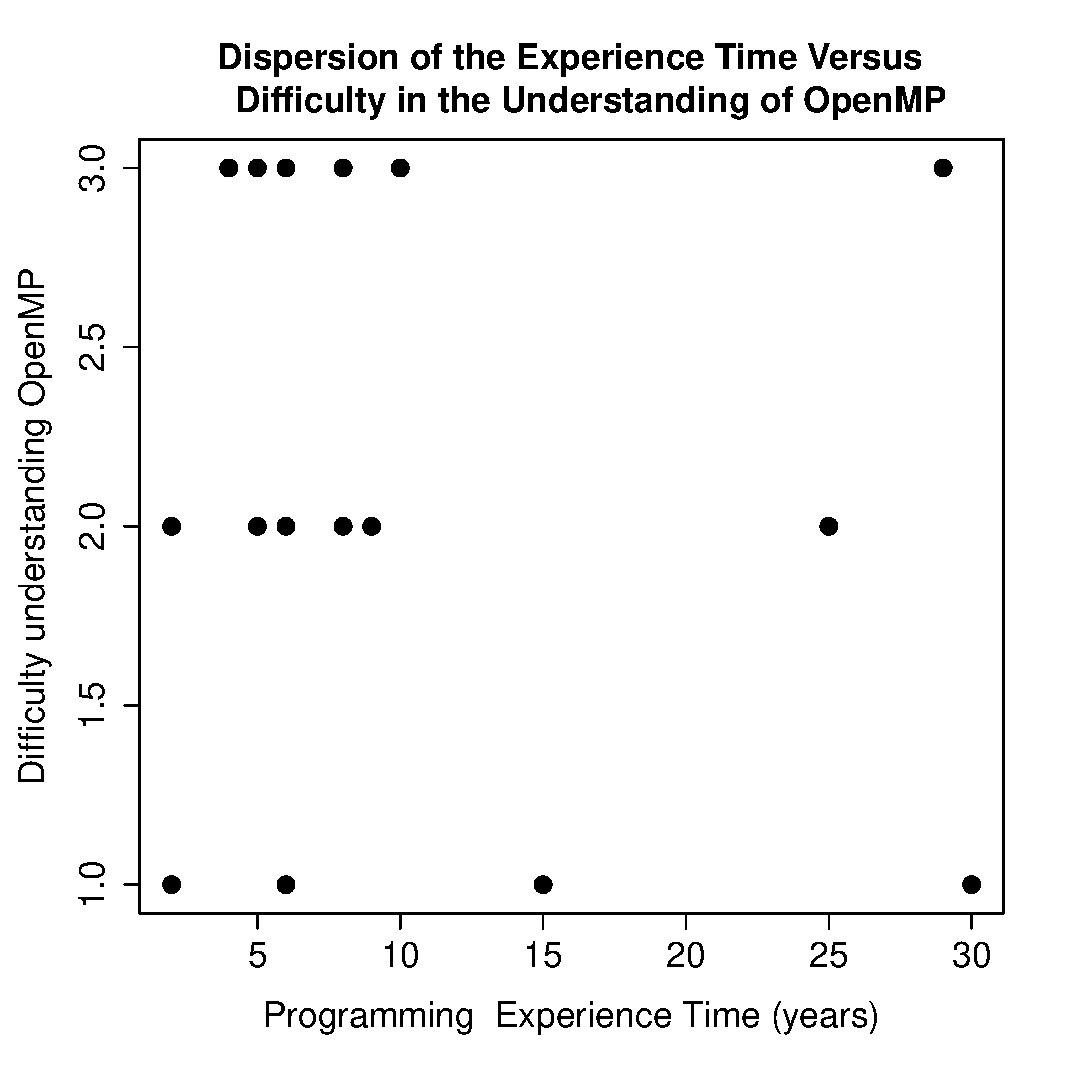
\includegraphics[width=0.95\columnwidth,height=0.9\columnwidth]{figures/experience.eps}
\caption{Graphic of dispersion of the experience time versus
    difficulty in the understanding of OpenMP}
\label{fig:DifOpenMP}
\end{figure}



\begin{comment}
Talvez seja importante falar também que os alunos tiveram aulas sobre conceitos de paralelismo antes.

Qual opinião você pode dar sobre sua experiência com \texttt{OpenMP} e sobre o Exercício de Programação 1?

1. Legal.

2. Achei interessante a ideia de anotar um programa que já funciona sequencialmente, mas esse método dificulta um pouco pensar em paralelo. Quando implementamos explicitamente as threads, tenho a impressão de que fica mais fácil entender os possíveis problemas.

3. Não conhecia o \texttt{OpenMP}, aparentemente é uma boa ferramenta, com alguma facilidade de aprendizado e já tenho utilizado para processamento de dados GPS sem maiores dificuldades. Sobre o EP1, aparentemente não trouxe grandes problemas técnicos. Apenas acho que, para efeito de aprendizado, ao invés de utilizar um grande problema, fosse mais conveniente propor mais pequenos problemas que servissem para salientar tópicos específicos.

4. Gostei bastante do EP1 por que o foco estava mais na compreensão de paralelismo e concorrência e menos num algoritmo complexo. Testes de desempenho sempre são divertidos e interessantes (comparação, interpretação).

5. Acredito que o EP1 foi bastante útil para o aprendizado das API do \texttt{OpenMP} para a utilização na prática.

6. Foi uma experiência interessante. Nunca tinha usado uma API de alto nivel. Só tinha usado semáforos e mutex. Gostei o fato que o \texttt{OpenMP} faz que, com pouco esforço, uma aplicação se torne paralela.

7. A implementação foi bem fácil (porque o problema era bem simples) e deu espaço para experimentarmos um pouco com as comparações e gráficos dos resultados; funcionou muito bem.

8. A utilização do \texttt{OpenMP} é bastante simples comparada com o uso de threads ou troca de mensagens como MPI (as duas outras ferramentas para programação paralela que eu tinha experiência anteriormente). Porém, os mesmos cuidados com deadlocks, granularidade, barreiras e etc. valem para o \texttt{OpenMP} também.

9. Foi instrutivo utilizar o \texttt{OpenMP}, apredner um outro método de fazer paralelismo

10. Enquanto estudava \texttt{OpenMP} fiquei pensando "por que raios isso não foi visto depois de pthread em Concorrente?".

11. Os exercícios foram simples de entender e nos permitiram avaliar a razão dos resultados obtidos.

12. Achei legal a experiência de ver a comparação de desempenho por processador e por número de threads. Outra coisa que gosto é a parte de focar mais no conceito e seu entendimento. EP simples que tocava exatamente no conceito me parece melhor que um EP super trabalhoso que talvez desse trabalho em pontos não relevantes à disciplina.

13. Quanto à \texttt{OpenMP} as dificuldades são relacionadas a: - corretude: será que nenhum caso foi esquecido (algo comum em paralelismo)? - otimização: será que a escolha foi a melhor possível para a implementação?
Quanto ao EP1, as dificuldades foram:
A maior dificuldade foi no exercício 1. Foi difícil definir uma estratégia para avaliar os códigos encontrados: compilar e executá-los poderia trazer problemas mais rápidos mas tomaria mais tempo um por um enquanto que avaliar somente analisando o código era mais difícil encontrar erros em um dado exemplo mas era possível analisar mais códigos. Quanto ao exercício 2, a dificuldade foi encontrar máquinas com arquiteturas diferentes. A menos que vc esteja envolvido em alguma área de computação científica ou paralela, a grande maioria dos computadores são x86.

14. Foi uma experiência positiva. Uma boa introdução a paralelização, que mostrou o quanto é prático usar \texttt{OpenMP}, pelo menos para uma aplicação simples como a do EP1. O problema em questão era suficientemente interessante para pensar nas questões do paralelismo por permitir várias formas de abordagem, e as ferramentas básicas do \texttt{OpenMP} foram suficientes para os experimentos e discussões.

15. Essa experiência me encorajou a usar o \texttt{OpenMP} em programas que eu venha a escrever e que sejam fáceis de paralelizar."

16. Tive contanto com conceitos de paralelismo no meu curso de graduação inclusive utilizando o \texttt{OpenMP}, porém a experiência da utilização do \texttt{OpenMP} neste trabalho foi muito melhor. Acho que senti bastantante a diferença neste EP1 por partirmos de uma versão sequencial, diferentemento do trabalho que fiz na graduação e o \texttt{OpenMP} se mostrou muito bem nesta situação.

17. O \texttt{OpenMP} é muito fácil de aprender mas há códigos com erros na internet, geralmente esses códigos tinham erros na operação "cout" do c++, geralmente usam ele para mostrar dados dentro de uma região paralela, pareceria que não sabem que essa operação não é atómica, outros tipos de erros que achei foram erros no código, por exemplo o erro mais comum que eu vi foram que eles não verificam se o indice de um arranjo é valido ou não; quer dizer que alguns tutoriais tem erros no mesmo algoritmo não verificam se o algoritmo é correcto ou não.

18. Foi o primeiro contato que tive com \texttt{OpenMP}. Achei bastante proveitoso aprender a utilizar o \texttt{OpenMP}. Além disso, foi divertido fazer experimentos para avaliar o desempenho do programa usando diferentes implementações.

19. O \texttt{OpenMP} me parece um bom framework para produtividade, ou seja, permite a criação de programas concorrentes em menos tempo e com menos código do que com pthreads, por exemplo, mas não torna a programação paralela uma tarefa trivial ou livre de erros.

20. "O \texttt{OpenMP} oferece uma sintaxe concisa para resolver um problema complexo. Dominar o poder que a interface proporciona requer um tempo considerável de estudo e reflexão para se chegar ao resultado esperado, portanto trata-se muito mais de um exercício intelectual do que mecânico.
A sintaxe tem uma carga conceitual muito grande. Tenho experiência em trabalhar com outras linguagens que têm características semelhantes de concisão e carga conceitual (por exemplo, Ruby) e acredito que leva um tempo relativamente mais alto para se obter proficiência nesse tipo de tecnologia, quando comparado com tecnologias de mais baixo nível. Mas o ganho de produtividade é indiscutível.
Sobre o EP1, achei que foi bem dimensionado para o conteúdo apresentado em aula. O que acredito que poderia ajudar é colocar exemplos de código para análise de desempenho e de scripts para coletar os dados obtidos, de forma a proporcionar foco no \texttt{OpenMP} para os estudantes desenvolverem o trabalho."

21. Gostei do desenvolvimento do programa sugerido(exerc.2 programa mult.c). Mas não gostei do exercício de procurar códigos errados na internet(exerc. 1). Gostaria de ter tido mais exercícios programando, analisando performance, etc... Ou seja, acho que poderíamos ter explorado melhor a tecnologia, fazendo mais códigos e análise de performance.

22. Achei muito interessante o desenvolvimento do EP1. Ajudou a mostrar a facilidade do uso do \texttt{OpenMP}, conseguindo melhoras significativas de performance com pequenas mudanças no código.

23. Toma tempo acostumbrar ao troco de programas sequenciais para os paralelos, mas com \texttt{OpenMP} não foi muito dificil porque só tem que colocar algumas linhas de código e o programa se faz paralelo (mas igual tem que ter cuidado algumas vezes).

24. Tive pouca experiência com \texttt{OpenMP} e pthreads, mas acredito que o entendimento de pthreads é mais fácil para quem já tem experiência em C. As barreiras implícitas me confundem porque nunca tenho certeza se existe barreira ou não.

\end{comment}

\section{Conclusions and next steps}
\label{sec:conclusions}

This paper's results reiterate that, even though \texttt{OpenMP} can be easy to use, programmers still need to know the details about parallel computing architectures and platforms. Teaching and learning the fundamental concepts about parallel programming is, and will continue to be, necessary to write accurate and high-performance code.

The experimental results show that although Internet tutorials transmit the idea of ease-of-use of the compilation directives approach, the core concepts of parallelism are required to write good parallel programs. Knowing the underlying platform and architectural details, and what effects are caused by directives and their interactions is also required.

Using \texttt{OpenMP} for trivial programs is easy, but for more advanced applications it is necessary to know how to correctly use locks and barriers, avoid deadlocks, and distribute the work evenly between threads. The programmer also has to be cautious when scheduling and accessing memory. To do all this correctly it is necessary to learn the fundamental concepts underlying parallel programming.

The main goal of parallel programming is writing programs that are efficient, portable and correct, leveraging contemporary hardware platforms~\cite{Asanovic2009}. These goals are still hard to reach even when using high-level approaches such as \texttt{OpenMP}.

It is important to teach Computer Science students how to program parallel applications from the beginning. Instead of teaching sequential programming first and parallel programming much later in the graduation course, Computer Science courses should start with \texttt{OpenMP} or other high-level tools, but not before providing solid fundamentals in parallel computing.

Considering the students' answers, a positive outcome of this experiment is that the students have learned that they should not rely on copying code from the Internet, because they can contain errors. Students also learned that they should test their code thoroughly, as errors in parallel programs are not easily detectable.

Future work will repeat the experiment in other instances of the graduate course, improving the experiment data set. Using a more systematic approach, future work will look for possible errors in more tutorials available on the Internet, and explore the difficulties faced by beginner and expert developers of parallel applications.

Finally, considering the results presented in this paper and the fact that even those who are teaching make mistakes in their tutorials and classes, more attention has to be devoted to teaching parallel and concurrent programming, its techniques, concepts and tools.


% An example of a floating figure using the graphicx package.
% Note that \label must occur AFTER (or within) \caption.
% For figures, \caption should occur after the \includegraphics.
% Note that IEEEtran v1.7 and later has special internal code that
% is designed to preserve the operation of \label within \caption
% even when the captionsoff option is in effect. However, because
% of issues like this, it may be the safest practice to put all your
% \label just after \caption rather than within \caption{}.
%
% Reminder: the "draftcls" or "draftclsnofoot", not "draft", class
% option should be used if it is desired that the figures are to be
% displayed while in draft mode.
%
%\begin{figure}[!t]
%\centering
%\includegraphics[width=2.5in]{myfigure}
% where an .eps filename suffix will be assumed under latex, 
% and a .pdf suffix will be assumed for pdflatex; or what has been declared
% via \DeclareGraphicsExtensions.
%\caption{Simulation Results}
%\label{fig_sim}
%\end{figure}

% Note that IEEE typically puts floats only at the top, even when this
% results in a large percentage of a column being occupied by floats.


% An example of a double column floating figure using two subfigures.
% (The subfig.sty package must be loaded for this to work.)
% The subfigure \label commands are set within each subfloat command, the
% \label for the overall figure must come after \caption.
% \hfil must be used as a separator to get equal spacing.
% The subfigure.sty package works much the same way, except \subfigure is
% used instead of \subfloat.
%
%\begin{figure*}[!t]
%\centerline{\subfloat[Case I]\includegraphics[width=2.5in]{subfigcase1}%
%\label{fig_first_case}}
%\hfil
%\subfloat[Case II]{\includegraphics[width=2.5in]{subfigcase2}%
%\label{fig_second_case}}}
%\caption{Simulation results}
%\label{fig_sim}
%\end{figure*}
%
% Note that often IEEE papers with subfigures do not employ subfigure
% captions (using the optional argument to \subfloat), but instead will
% reference/describe all of them (a), (b), etc., within the main caption.


% An example of a floating table. Note that, for IEEE style tables, the 
% \caption command should come BEFORE the table. Table text will default to
% \footnotesize as IEEE normally uses this smaller font for tables.
% The \label must come after \caption as always.
%
%\begin{table}[!t]
%% increase table row spacing, adjust to taste
%\renewcommand{\arraystretch}{1.3}
% if using array.sty, it might be a good idea to tweak the value of
% \extrarowheight as needed to properly center the text within the cells
%\caption{An Example of a Table}
%\label{table_example}
%\centering
%% Some packages, such as MDW tools, offer better commands for making tables
%% than the plain LaTeX2e tabular which is used here.
%\begin{tabular}{|c||c|}
%\hline
%One & Two\\
%\hline
%Three & Four\\
%\hline
%\end{tabular}
%\end{table}


% Note that IEEE does not put floats in the very first column - or typically
% anywhere on the first page for that matter. Also, in-text middle ("here")
% positioning is not used. Most IEEE journals/conferences use top floats
% exclusively. Note that, LaTeX2e, unlike IEEE journals/conferences, places
% footnotes above bottom floats. This can be corrected via the \fnbelowfloat
% command of the stfloats package.



%\section{Conclusion}
%The conclusion goes here.

% conference papers do not normally have an appendix


% use section* for acknowledgement
%\section*{Acknowledgment}

%The authors would like to thank...

\section*{Acknowledgments}
\label{sec:acknowledgments}

The authors would like to thank Students who participated in this exercise ...



% trigger a \newpage just before the given reference
% number - used to balance the columns on the last page
% adjust value as needed - may need to be readjusted if
% the document is modified later
%\IEEEtriggeratref{8}
% The "triggered" command can be changed if desired:
%\IEEEtriggercmd{\enlargethispage{-5in}}

% references section

% can use a bibliography generated by BibTeX as a .bbl file
% BibTeX documentation can be easily obtained at:
% http://www.ctan.org/tex-archive/biblio/bibtex/contrib/doc/
% The IEEEtran BibTeX style support page is at:
% http://www.michaelshell.org/tex/ieeetran/bibtex/
\bibliographystyle{IEEEtran}
% argument is your BibTeX string definitions and bibliography database(s)
\bibliography{IEEEabrv,ref}

%
% <OR> manually copy in the resultant .bbl file
% set second argument of \begin to the number of references
% (used to reserve space for the reference number labels box)
%\begin{thebibliography}{1}

%\bibitem{IEEEhowto:kopka}
%H.~Kopka and P.~W. Daly, \emph{A Guide to \LaTeX}, 3rd~ed.\hskip 1em plus
%  0.5em minus 0.4em\relax Harlow, England: Addison-Wesley, 1999.

%\end{thebibliography}

% that's all folks
\end{document}
